\documentclass{article}

\title{Algebraic Topology Homework 4}
\author{Adam Buskirk}

\usepackage{amssymb,amsmath,amsthm}
\usepackage{tikz}
\usetikzlibrary{trees}
\usetikzlibrary{matrix}
\usepackage[margin=1in]{geometry}

\newtheorem{theorem}[subsection]{Theorem}
\newtheorem{conjecture}[subsection]{Conjecture}
\newtheorem{lemma}[subsection]{Lemma}
\theoremstyle{definition}
\newtheorem{definition}[subsection]{Definition}

\newcommand{\R}{\mathbb{R}}
\newcommand{\N}{\mathbb{N}}
\newcommand{\Q}{\mathbb{Q}}
\newcommand{\Z}{\mathbb{Z}}
\newcommand{\Co}{\mathbb{C}}
\newcommand{\p}[1]{\left(#1\right)}
\newcommand{\sq}[1]{\left[#1\right]}
\newcommand{\set}[1]{\left\{#1\right\}}
\newcommand{\norm}[1]{\left|\left|#1\right|\right|}
% \newcommand{\p}[1]{\left(#1\right)}

\begin{document}
\maketitle

\section{Problem 2}
\begin{theorem}
Let $X=\R^{n+1} \setminus \{0\}$; define an equivalence relation on 
$\sim$ on $X$ where $x \sim y$ iff $x=\lambda y$ for some $\lambda \in \R^+$.
Then $S^n \cong X/\sim$. Furthermore we can define another equivalence
relation $\bumpeq$ on $S^n$ by identifying antipodal points and show that
$S^n/\bumpeq \cong \R P^n$.
\end{theorem}
\begin{proof}
Let $q : x \mapsto [x]_\sim$ be the quotient map which takes each element of
$\R^{n+1} \setminus\{0\}$ to its equivalence class under $\sim$, and let 
$f : X \to S^n$, $f : x \mapsto \frac{1}{|x|} x$.
{\begin{center}
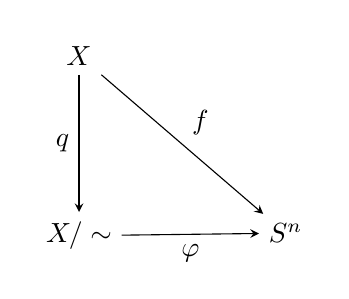
\begin{tikzpicture}[every node/.style={midway},->,>=stealth]
        \matrix (m) [matrix of math nodes, column sep={5em}, row sep={5em}]
        {
                X & \\
                X / \sim & S^n
        \\};
        \draw[->] (m-1-1) -- (m-2-2) node[above right] {$f$} ;
        \draw[->] (m-1-1) -- (m-2-1) node[left] {$q$};
        \draw[->] (m-2-1) -- (m-2-2) node[below] {$\varphi$};
\end{tikzpicture}
\end{center}}
The map $f$ is constant on the fibers of $q$, since if $f(x_1) = f(x_2)$ then
$x_1/|x_1|=x_2/|x_2|$, which implies $x_1 = \frac{|x_1|}{|x_2|} x_2$, meaning
$x_1 \sim x_2$ and thus $q(x_1) = q(x_2)$. On the other hand, if 
$q(x_1)=q(x_2)$ then $x_1=\lambda x_2$, so $|x_1|=\lambda |x_2|$ which
implies $\lambda = \frac{|x_1|}{|x_2|}$ and thus 
$x_1 = \frac{|x_1|}{|x_2|} x_2$ and so 
$f(x_1) = x_1/|x_1| = x_2 / |x_2| = f(x_2)$.
Thus by Theorem 3.75
there must exist a homeomorphism $\varphi : X/\sim \to S^n$, and thus
$X/\sim$ and $S^n$ are homeomorphic.

Similarly, if we let $g$ map each point in $X$ to its equivalence class
in $\R P^n$, and let $p$ map each point of $S^n$ to the equivalence class
of antipodal points defined by $\bumpeq$, we have 
{\begin{center}
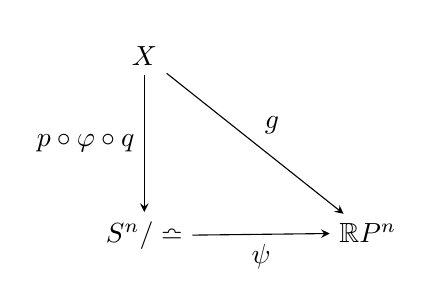
\begin{tikzpicture}[every node/.style={midway},->,>=stealth]
        \matrix (m) [matrix of math nodes, column sep={5em}, row sep={5em}]
        {
                X & \\
                S^n/\bumpeq & \R P^n
        \\};
        \draw[->] (m-1-1) -- (m-2-2) node[above right] {$g$} ;
        \draw[->] (m-1-1) -- (m-2-1) node[left] {$p\circ \varphi \circ q$};
        \draw[->] (m-2-1) -- (m-2-2) node[below] {$\psi$};
\end{tikzpicture}
\end{center}}
If $g(x_1) = g(x_2)$ then $x_1 = \lambda x_2$ so 
$|x_1| = |\lambda| \cdot |x_2|$ so $|\lambda| = \frac{|x_1|}{|x_2|}$. 
Hence $x_1 = s\frac{|x_1|}{|x_2|} x_2$ for some $s \in \{-1,1\}$, whichever
is appropriate. If $s=1$, then $\varphi \circ q = f$ maps $x_1$ and $x_2$
to the same element, and thus 
$p \circ \varphi \circ q (x_1) = p \circ \varphi \circ q (x_2)$. $s=-1$, then
they map to opposite points on the sphere, which are in the same equivalence
class, and thus the same equality holds. 

If $p \circ \varphi \circ q (x_1) = p \circ \varphi \circ q (x_2)$, then 
$\varphi \circ q (x_1) = \pm \varphi \circ q (x_2)$ which is the same
as $f (x_1) = \pm f(x_2)$ and thus $x_1/|x_1| = \pm x_2 / |x_2|$, so 
$x_1 = \pm \frac{|x_1|}{|x_2|} x_2$ so $x_1 \bumpeq x_2$ and thus
$g(x_1) = g(x_2)$.

Since both maps agree on fibers, by 3.75 there exists a homeomorphism 
$\psi$ between $S^n / \bumpeq$ and $\R P^n$.
\end{proof}

\section{Problem 3}
\begin{theorem}
Let $X=\R \times \{0,1\}$, and let $\sim$ such that $(x,1) \sim (y,0)$ iff 
$x=y \neq 0$. Therefore, the classes $[(0,0)]$ and $[(0,1)]$ are distinct.
Then $X / \sim$ is second countable, locally Euclidean, but not Hausdorff.
\end{theorem}
\begin{proof}
$X$ is second countable, and thus $X / \sim$ must be. Any point of $X$ 
permits open $U_x \cong B^n$. Thus, for any point in $X/ \sim$ except
the two origins, we have an open neighborhood homeomorphic to $B^n$ 
descended from the neighborhoods yielded by that point's preimages;
either of these two will work. Either origin also carries its own open
neighborhood down through the quotient map.

However, $X / \sim$ is not Hausdorff, since we cannot find disjoint 
open balls around $[(0,0)]$ and $[(0,1)]$. The preimage of a neighborhood
of $[(0,0)]$ must contain some open interval $(a,b) \times \{0\}$,
and also the preimage of a neighborhood of $[(0,1)]$ must contain
some $(c,d) \times \{1\}$. However, consider the points 
$(\min(b,d)/2,0)$ and $(\min(b,d)/2,1)$; since neither $b$ nor $d$ can
be $0$, these must map to the same point under the quotient map. 
Consequently, the neighborhoods around $[(0,0)]$ and $[(0,1)]$ are
not disjoint; but they were chosen arbitrarily, and thus disjoint
open neighborhoods for these points in $X / \sim$ cannot be found.
Consequently, $X / \sim$ is not Hausdorff.
\end{proof}
\section{Problem 4}
\section{Problem 5}
\begin{theorem}
Manifolds have countably many connected components.
\end{theorem}
\begin{proof}
Suppose a manifold had uncountably many connected components. Since each
of these is an open set, for any basis for the manifold's topology, 
each of these connected components must contain a distinct basis
element. Thus an injection may be made from the uncountable collection
of components into any basis for the manifold, and thus any basis
for the manifold must be uncountable, contradicting the requirement
that a manifold be second-countable.
\end{proof}
\section{Problem 6}
\begin{theorem}
Let $G$ be a topological group and let $e$ denote the identity element. 
Let $H$ denote the connected component containing $e$. Then $H$ is a 
subgroup.
\end{theorem}
\begin{proof}
Consider arbitrary $g, h \in H$, and consider $\Phi_h : H \to G$ defined
by $\Phi_h ( k ) = kh^{-1}$. Then $\Phi_h$ is constructed from three 
different operations. First, $h \to h^{-1}$ is continuous by the definition
of a topological group. Also, the restriction of the product to $H \times H$
is continuous. So the composition $\phi : (j,k) \in H^2 \mapsto j \cdot k^{-1}G$ 
is continuous. So then $\Phi_h (k) = \phi(k,h)$ is continuous. Thus, since
continuous maps preserve connectivity by Theorem 4.7 in the text, we know that
$\Phi_h(H)$ is a connected set. Furthermore, 
$\Phi_h(h) = h h^{-1} = e \in \Phi_h(H)$,
so $\Phi_h(H) \subseteq H$; if not, $H$ would not be maximal, since 
$\phi_h(H) \cup H$ would then be a larger connected set not disjoint from $H$, 
and thus $H$ would not be considered a connected component of $G$. Since 
$g \in H$, the domain of $\Phi_h$, then 
$gh^{-1} = \Phi_h (g) \in \Phi_h (H) \subset H$, so $gh^{-1} \in H$. Thus,
$H$ is a subgroup of $G$.
\end{proof}

\end{document}
